\chapter{Bilderkennung}
\label{bilderkennung}
Bei dem Bildverarbeitungsprozess muss das Paket vor verschiedenen Hintergründen, erkannt werden. Dabei darf die Beleuchtung keine Rolle spielen. Die charakteristischen Eigenschaften sind neben Farbe somit ebenfalls Form und Größe.

Zuerst wurde RGB(Red, Green, Blue) Farbraum gefiltert. Jedoch ergaben Test's das der RGB-Farbraum sehr belichtungsempfindlich ist. Deswegen wird das Bild in den HSV(Hue, Saturation, Value) Farbraum konvertiert. Dieser ist deutlich belichtungsstabiler.
\begin{figure}[h]
	\begin{center}
	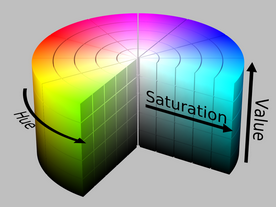
\includegraphics[scale=0.5]{"Grafiken/hsv_colorspace_zoom34.png"}
	\caption{HSV-Raum \\Quelle: https://www.cti-modellbau.de/CTI-Hubzylinder/titan/}
	\label{fig:meine-grafik}
	\end{center}
\end{figure}
Als Farbe wäre Rot sehr geeignet, da es in unsere Umgebung sehr selten vorkommt. Allerdings gibt es keine Roten-Pakete. Außerdem ist Rot für eine Kamera sehr schwer zu erkennen, da es eine der Grundfarben ist und damit in fast jeder Farbe vorkommt. Deswegen wurde als Farbe weiß gewählt. Durch den Filter werden nun weiße Flächen weiß und der Rest wird schwarz. Da das Experiment auf einem dunklen Boden stattfindet, bietet sich dies an.

Weiterhin muss auf dem Paket mittig, ein weiteres schwarzes Viereck sein. Dies ist nötig um eine Orientierung bei naher Distanz zu gewährleisten. Befindet sich die Drohne nahe über dem Paket, so füllt es das komplette Kamerasichtfeld aus. Um sich nun orientieren zu können ist ein weiteres Viereck nötig. Dies muss mittig sein, da sich die Drohne im Verlauf des Anflugs parallel zu dem Rechteck ausrichtet. Damit bei allen Rotationen der Versatz immer gleich ist, muss es mittig sein. Dadurch kann man ihn in der Kameraregelung berücksichtigen.

Für die Form wird der Hought-Transformation verwendet. Bei dieser wird das Bild zuerst abgeleitet. Also werden Pixel neben den sich ein andersfarbiges befindet weiß und der Rest(Weiß neben Weiß, Schwarz neben Schwarz) wird schwarz. Nun sind die Kanten deutlich zu sehen. Anschließend wird durch jeden weißen Punkt eine Linie mit verschieden Anstiegen zwischen - unendlich und + unendlich gelegt. Schneidet man dabei mit der Linie einen anderen weißen Punkt, so wird sich diese Linie gemerkt. Linien, die durch mehrere weiße Punkte gehen werden, so als Linien detektiert. Der Algorithmus wird aus der OpenCV Bibliothek implementiert. Er hat die Komplexität: n! (n Fakultät). \cite{wenyu2007}

Anschließend wird das Bild nach Konturen durchsucht. Dabei sind nur die Konturen mit 4 Ecken von Bedeutung. Diese Konturen werden nun nach minimaler und maximaler Größe gefiltert. Die Intervallbreite variiert abhängig von der Flughöhe. Außerdem spielt die Auflösung der Kamera ein Rolle, diese ist 640*480p (\ref{kamera})

Von den gefilterten Rechtecken wird nun der Mittelpunkt berechnet. Ist mit einem Umkreis von 10 Pixeln bereits ein weiteres Rechteck gefunden worden, so wird das Rechteck verworfen. Dadurch ist sicher gestellt, dass Rechtecke nicht doppelt erkannt werden. Erfüllt ein Rechteck all diese Bedingungen so wird noch die Rotation der oberen Kante berechnet. Diese wird dann zusammen mit den Mittelpunktkoordinaten an den Controller über ROS weitergeleitet. Es ist das Problem aufgetreten, dass das Viereck um 45° gedreht war. In diesem Fall gibt es 2 oberste kanten und der Algorithmus erkennt schlimmstenfalls abwechselnd beide. Um dies zu vermeiden, wurde eine 2 Regel eingeführt. Es wir immer die oberste Kante genommen. Gibt es 2, so wird die Linke davon genommen. Da es nicht 2 Oberste und Linkeste geben kann, ist der Algorithmus so eindeutig definiert und terminiert.\cite{Lagunovsky1997}

Um die Rechenzeit zu verringern, wird das Bild auf 640x480 Pixel herunter skaliert, da dies für einfache Vierecke völlig ausreicht. Außerdem wird der Hough Algorithmus bewusst erst nach dem Filtern ausgeführt, da seine Komplexität fakultativ mit der Anzahl der erkannten Objekte ansteigt. Auf diesem Wege ist eine Auswertung mit mehr als 5 Frames pro Sekunde möglich, was unseren Anforderungen genügt.

Der Bildverarbeitungsprozess läuft in der Image Progressing Node. Er wird maximal mit 10 Hz ausgeführt. Das stellt sicher das der Pi nicht überlastet und noch genügend Rechenkapazität für die anderen Codes/Prozesse hat. Da die Drohne nicht zu schnell fliegt, reicht dieses Schrittweite aus um ein stabiles Systemverhalten des PT1-Glied(Regler mit proportionaler Vergrößerung erster Ordnung). Es wurde experimentell in der Gazebosimulation herausgefunden das bei dem PX-4 Controller sogar eine Geschwindigkeit von 3 HZ ausreichend würde, da die Änderungsraten klein sind 0.1. Diese 0.1 steht dafür das, wenn der Regler eine Abweichung von 1 m erkennt, er der Drohne als neue Zielkoordinaten nur Koordinaten gibt, die 0,1 m entfernt sind. Dadurch fliegt sie langsamer und kippt nicht so stark. Durch das kippen wird die Kamera bewegt und ändert somit ihren Winkel auf den Boden. Dadurch wiederum wird das Paket falsch erkannt. (siehe Kapitel \ref{fazit}) 